\section{\textit{Online Controlled Experiment}}

Também conhecido como Teste A/B ou simplesmente \textit{OCE}, é um experimento realizado no contexto \textit{online}. Esse tipo de investigação tem como objetivo analisar diferentes versões de \textit{software}, escolhendo métricas para comparar variantes de uma mesma funcionalidade e validar ideias sobre o desenvolvimento do produto (e.g., dispor os elementos de maneira diferente em uma página \textit{web} deve tornar determinada atividade mais rápida). A versão inicial, sem mudanças, é chamada de controle, e a atualizada, de tratamento \cite{fabijan_online_2020}.

Durante a utilização, os usuários são distribuídos entre essas diferentes versões, e, à medida que interagem com o produto, suas atividades são registradas e as métricas escolhidas são coletadas. A diferença entre esses valores, caso seja estatisticamente significativa e se a coleta de dados foi feita corretamente, muito provavelmente foi introduzida pelo tratamento \cite{kohavi_oce_and_ab_tests_2017}. Dessa forma, finaliza-se um fluxo contínuo de aprendizado, semelhante ao ciclo proposto pela metodologia \textit{Lean}. Esse ciclo já foi formalizado anteriormente na literatura e é apresentado na Figura \ref{fig:oce_lifecycle}.

\begin{figure}
    \centering
    \caption{\textit{The Experiment Lifecycle} }
    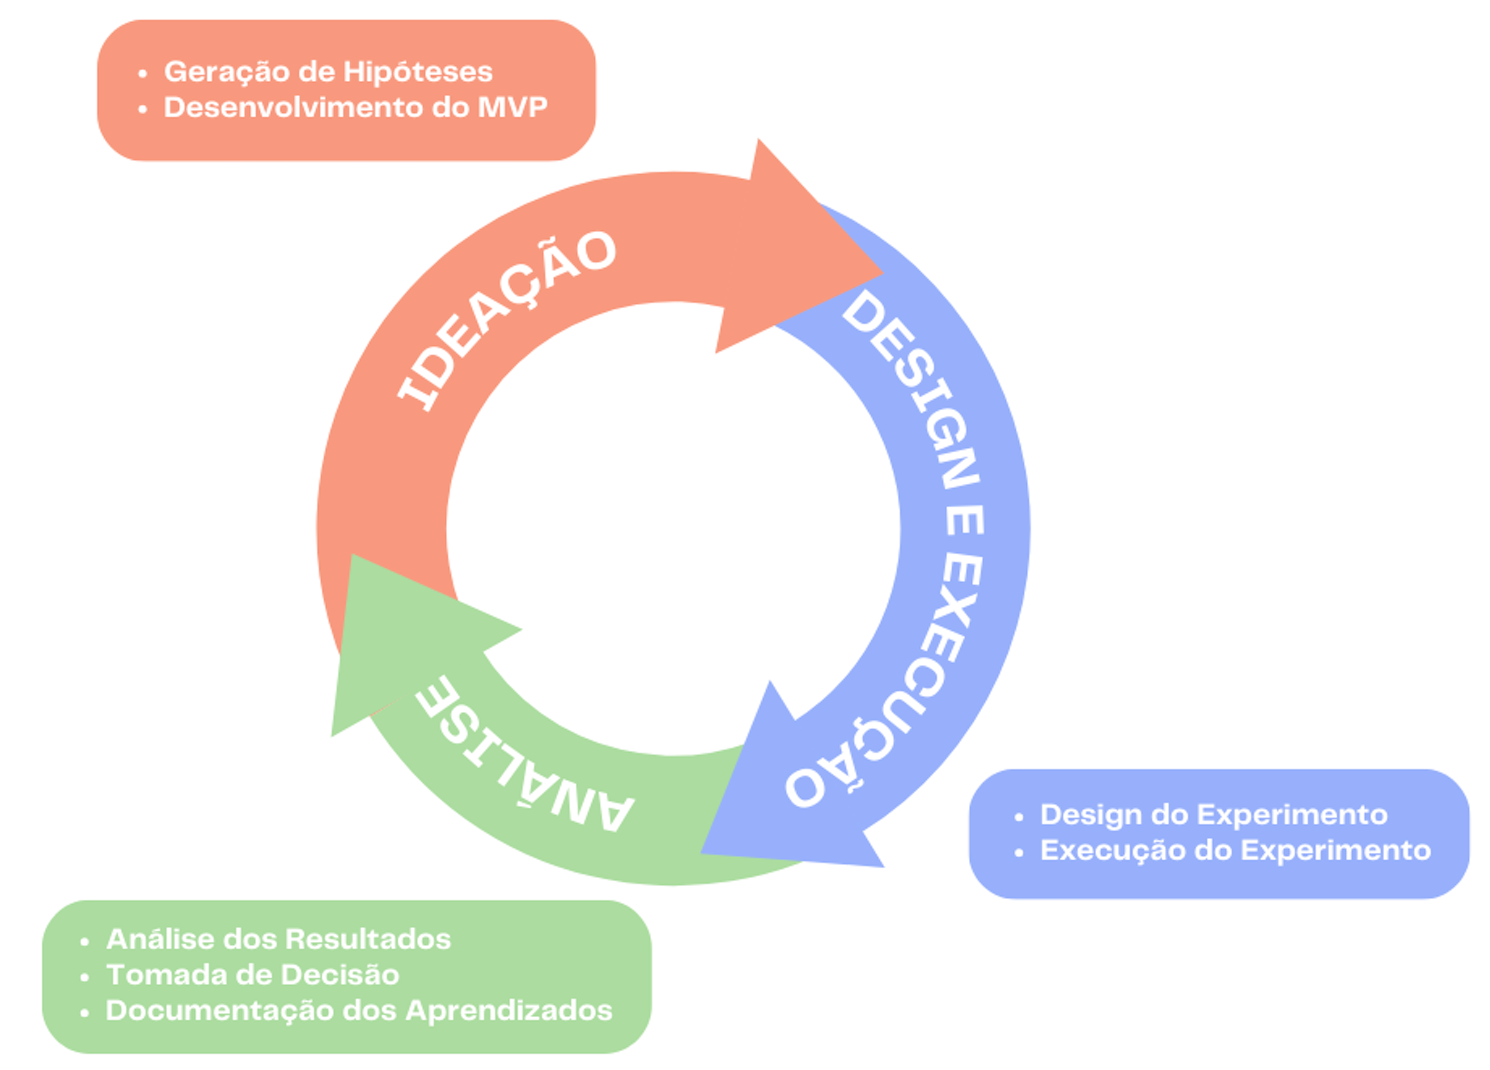
\includegraphics[width=0.75\linewidth]{figuras/oce_lifecycle.png}
    \text{Fonte: Adaptado de \citeonline{kohavi_online_2013}}
    \label{fig:oce_lifecycle}
\end{figure}
